\documentclass[UTF-8]{article}


\usepackage{booktabs}
\usepackage{url}
\usepackage{cite}
\usepackage[version=4]{mhchem}
\usepackage{graphicx}
\usepackage{subfigure}
\usepackage[a4paper,top=2cm,bottom=2cm,right=3cm,left=3cm,marginparwidth=1.75cm]{geometry}
%\usepackage[a4paper,top=2cm,bottom=2cm]{geometry}
\usepackage{amsmath}
\usepackage{upgreek}

\title{cGAS-STING Pathway in Innate Immune System}
\author{Yan Haoming}
\date{December 6\\ December 13\\ 2024}


\begin{document}
\maketitle

\section{Background}
As the first line of defense against pathogens, innate immune system is composed of protective barriers (epithelial surface) and \textbf{Pathogen Recognition Receptors (PRR)}\cite{TheCell}.
PRRs recognize \textbf{Pathogen-Associated Molecular Patterns (PAMP)} then activate intracellular signaling pathways.

\begin{table}[h]
    \centering
    \begin{tabular}{|c|c|}\hline
        \textbf{Abbreviations} & \textbf{Meanings} \\ \hline
        PAMP & Pathogen-Associated Molecular Patterns\\ \hline
        PRR & Pathogen Recognition Receptors \\ \hline
        cGAMP & cyclic GMP-AMP \\ \hline
        cGAS & cyclic GMP-AMP Synthase\\ \hline
        STING & Stimulator of Interferon Genes\\ \hline
        PBS & Phosphate-Buffered-Saline\\ \hline
        PFA & Paraformaldehyde\\ \hline
    
    \end{tabular}
    \caption{Terms their Abbreviations}
    \label{Terms}
\end{table}

In this context, PAMP refers to cytosolic DNA which is absent in normal cells.
Upon DNA recognition, \textbf{cGAS} dimerizes and stimulates the formation of \textbf{cyclic-GMP-AMP (cGAMP)}. cGAMP then binds directly to \textbf{stimulator of interferon genes (STING)} which triggers phosphorylation/activation of the transcription factor IRF3 via TBK1\cite{cGAS-wiki}.
The above pathway is visualized in Figure \ref{landscape}.

\begin{figure}[h]
    \centering
    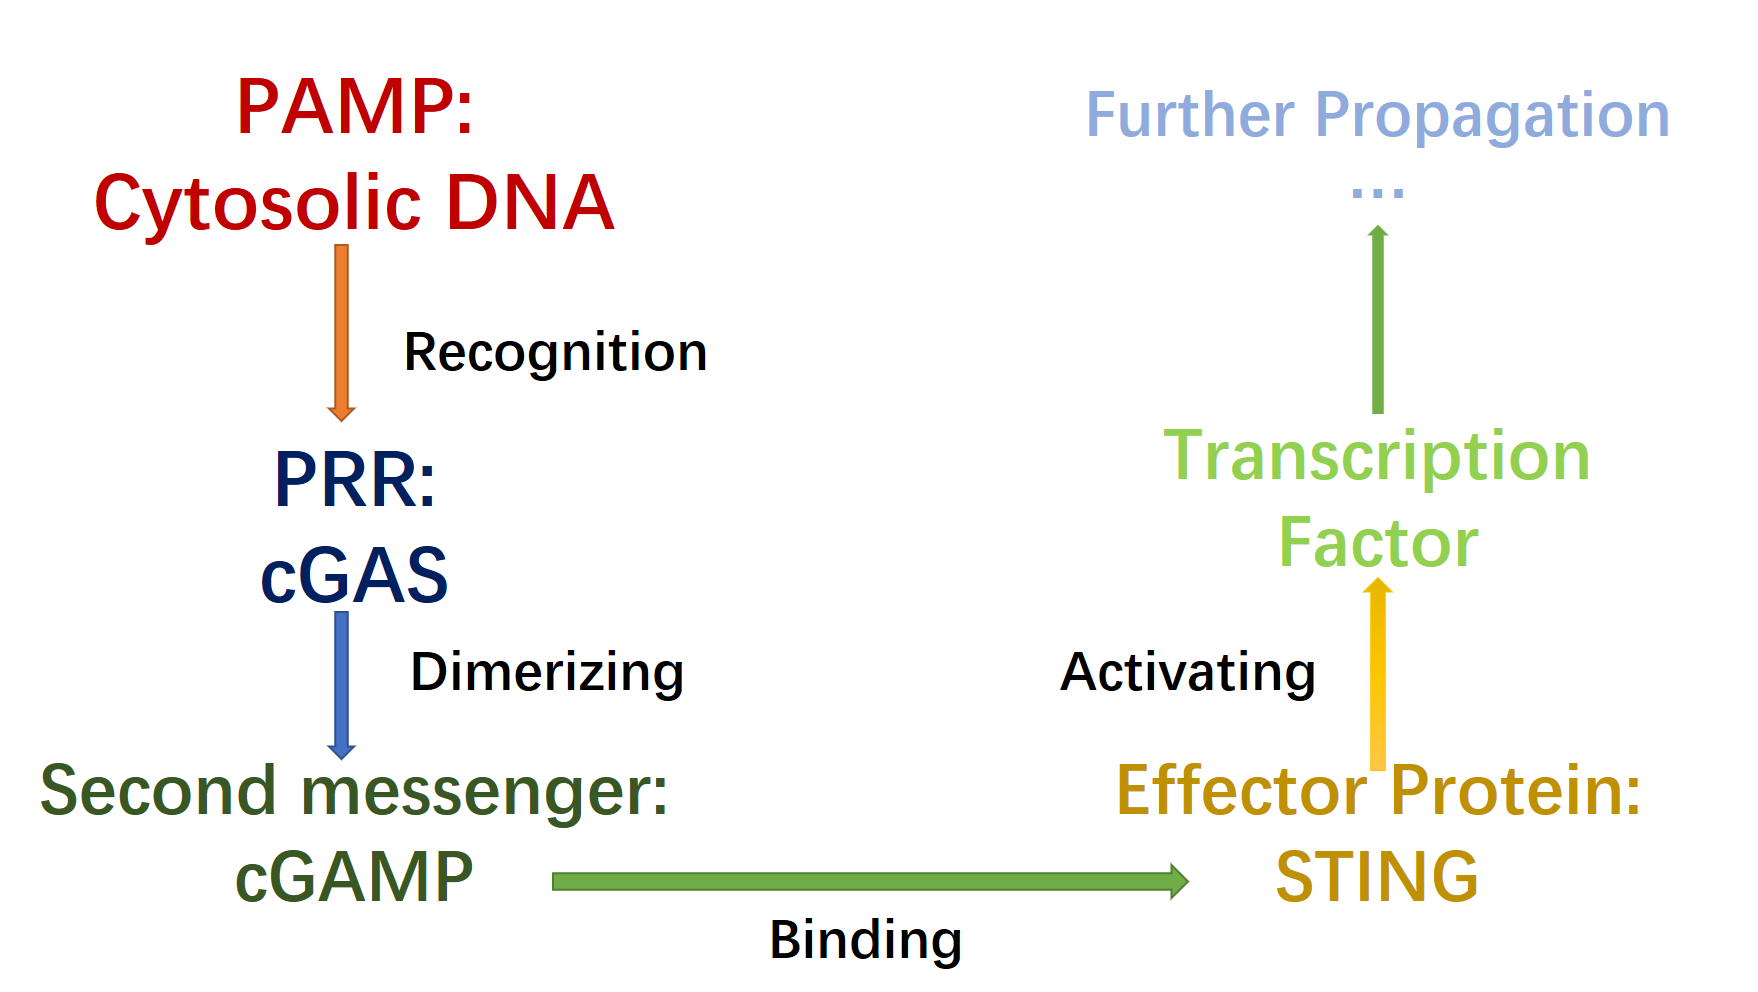
\includegraphics[width=0.7\linewidth]{../Figures/landscape.png}
    \caption{cCAS-STING Pathway in Innate Immune System}
    \label{landscape}
\end{figure}

The STING is initially confined at Endothelial Reticulum (ER) until activated by cGAMP.
With the signal of cGAMP, STING is transported to Golgi Apparatus or vesicular and forming a separated phase ,which helps gathering SING, for operating.
In this experiment, we focused on this transportation of STING by observing the different distribution of florescence labeled STING in the cells.

\section{Experimental Procedure}
In our experiment, the experimental group was treated by \textbf{diABZI (the chemical compound to activate cGAS-STING pathway)}, while the controlled group was not.
Hela cell line was used with GFP labelled STING.

We firstly transferred the cultured cells from its culture media to a microscope slide.
To achieve this, the following detailed procedure was performed:
\begin{itemize}
    \item remove liquid culture media by pipette.
    \item wash the cell by PBS (Phosphate-Buffered-Saline) 3 times, 500 $\upmu$L in around.
    \item add 500 $\upmu$L PFA (Paraformaldehyde) to both controlled group and experimental group.
    \item wait for 20 minutes for polymerization of PFA.
    \item add 6 $\upmu$L sealant to each group to prevent fluorescence quenching.
    \item seal the specimen by nail polish finally.
\end{itemize}

\section{Observations}
After a week we observed the specimen that we had manipulated using fluorescent light microscope.
The pictures captured under microscope are shown in Figure \ref{controlled group} and Figure \ref{Experimental group}.
 % Figure
 \begin{figure}[h]
    \centering
    \subfigure[capture 1]{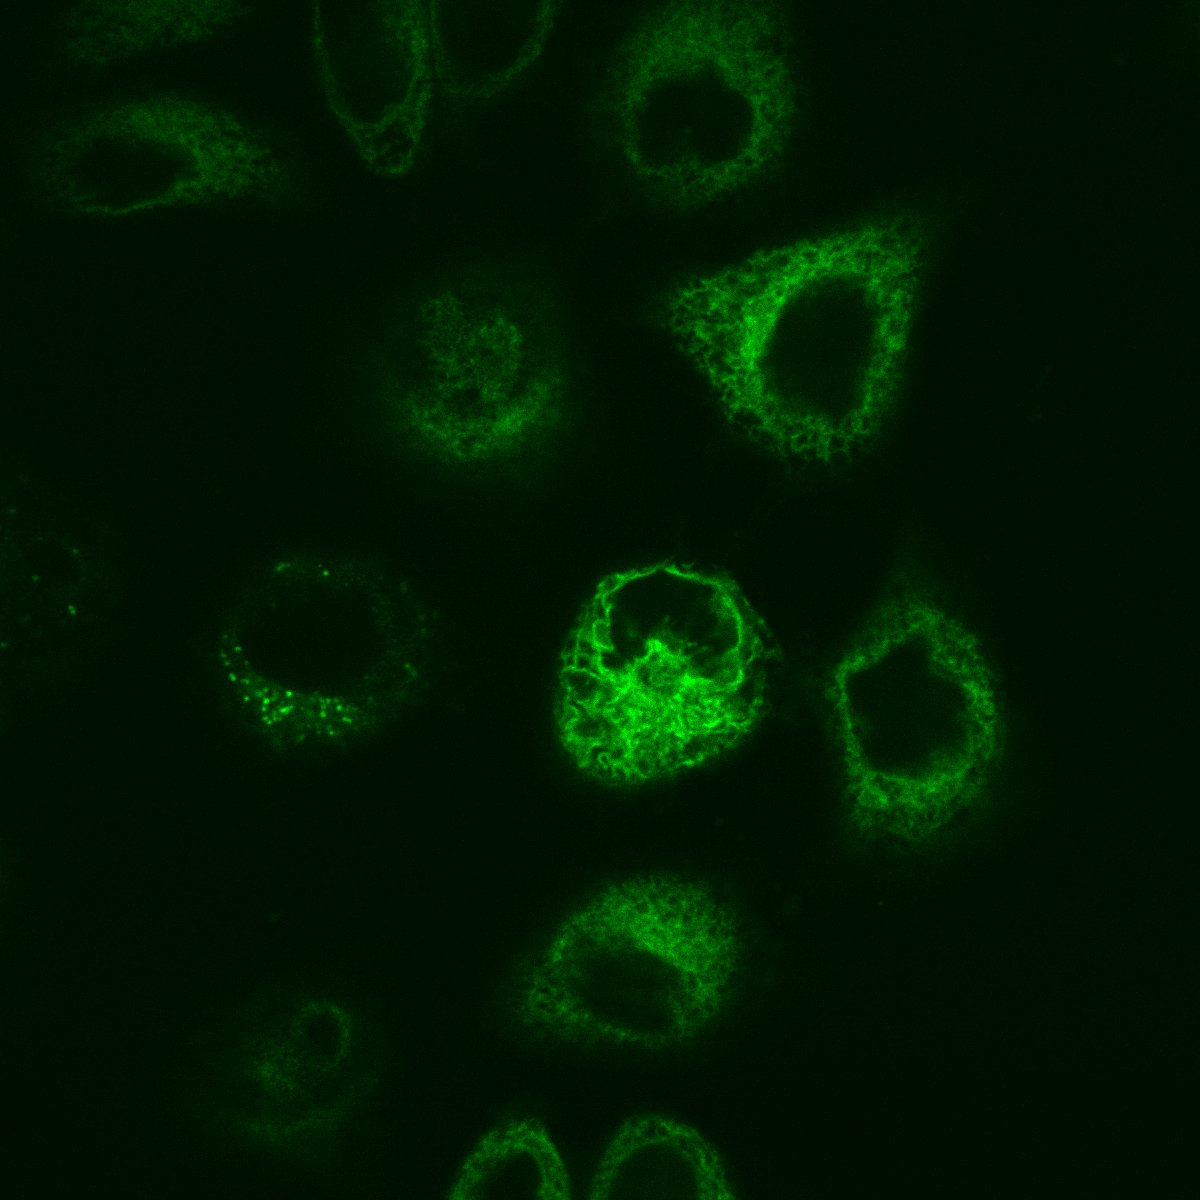
\includegraphics[width=0.3\linewidth]{../Figures/observations/G2 HeLa STING-GFP CON1.jpg}}
    \subfigure[capture 2]{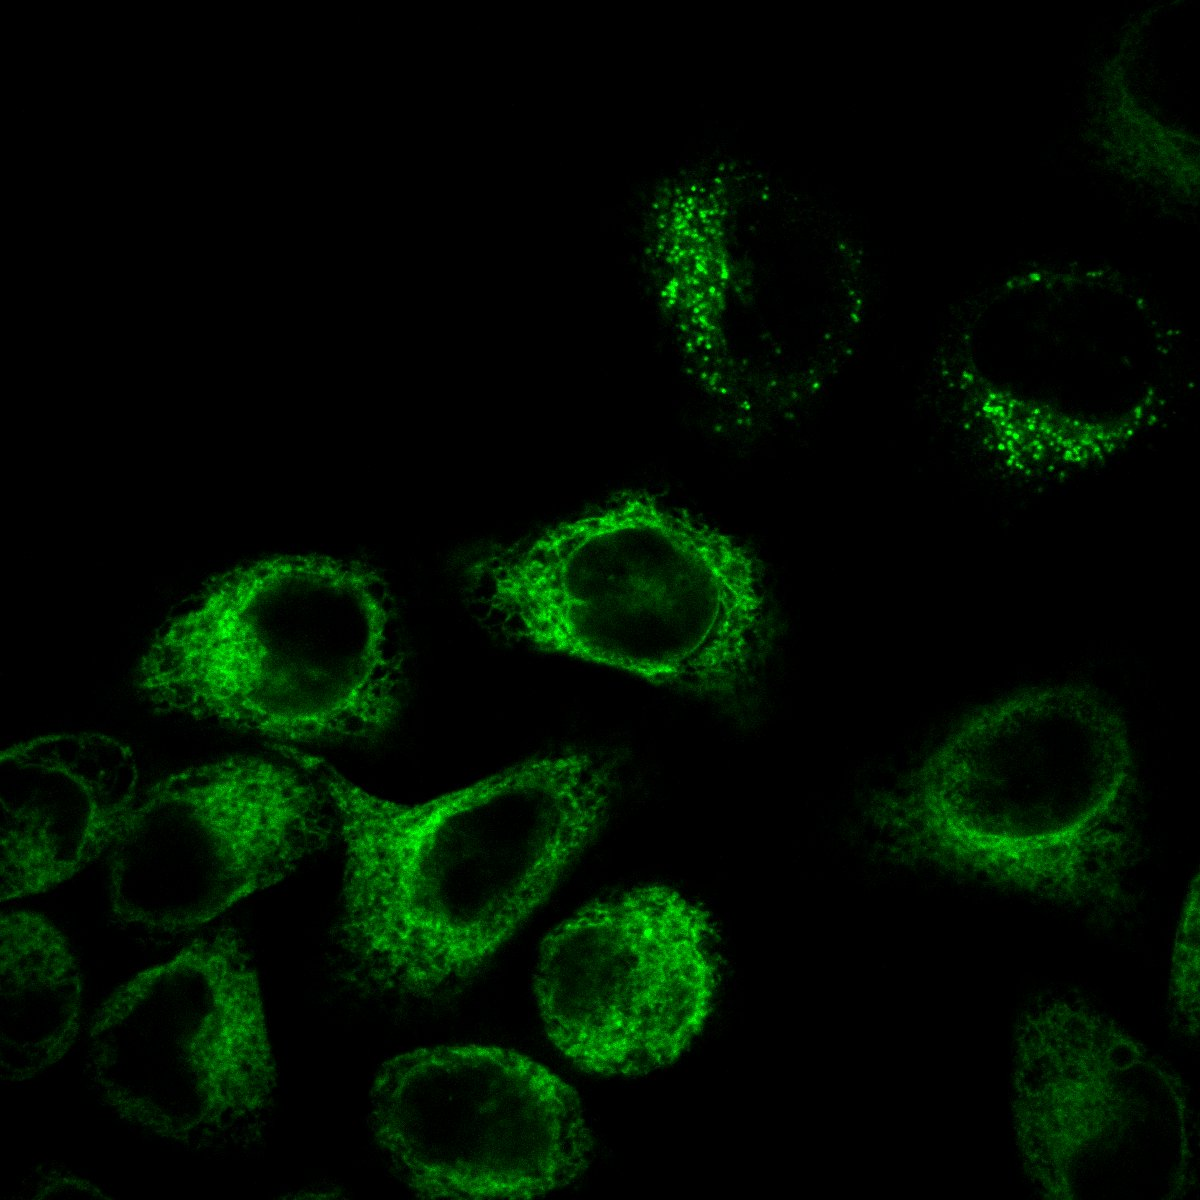
\includegraphics[width=0.3\linewidth]{../Figures/observations/G2 HeLa STING-GFP CON2.jpg}}
    \subfigure[capture 3]{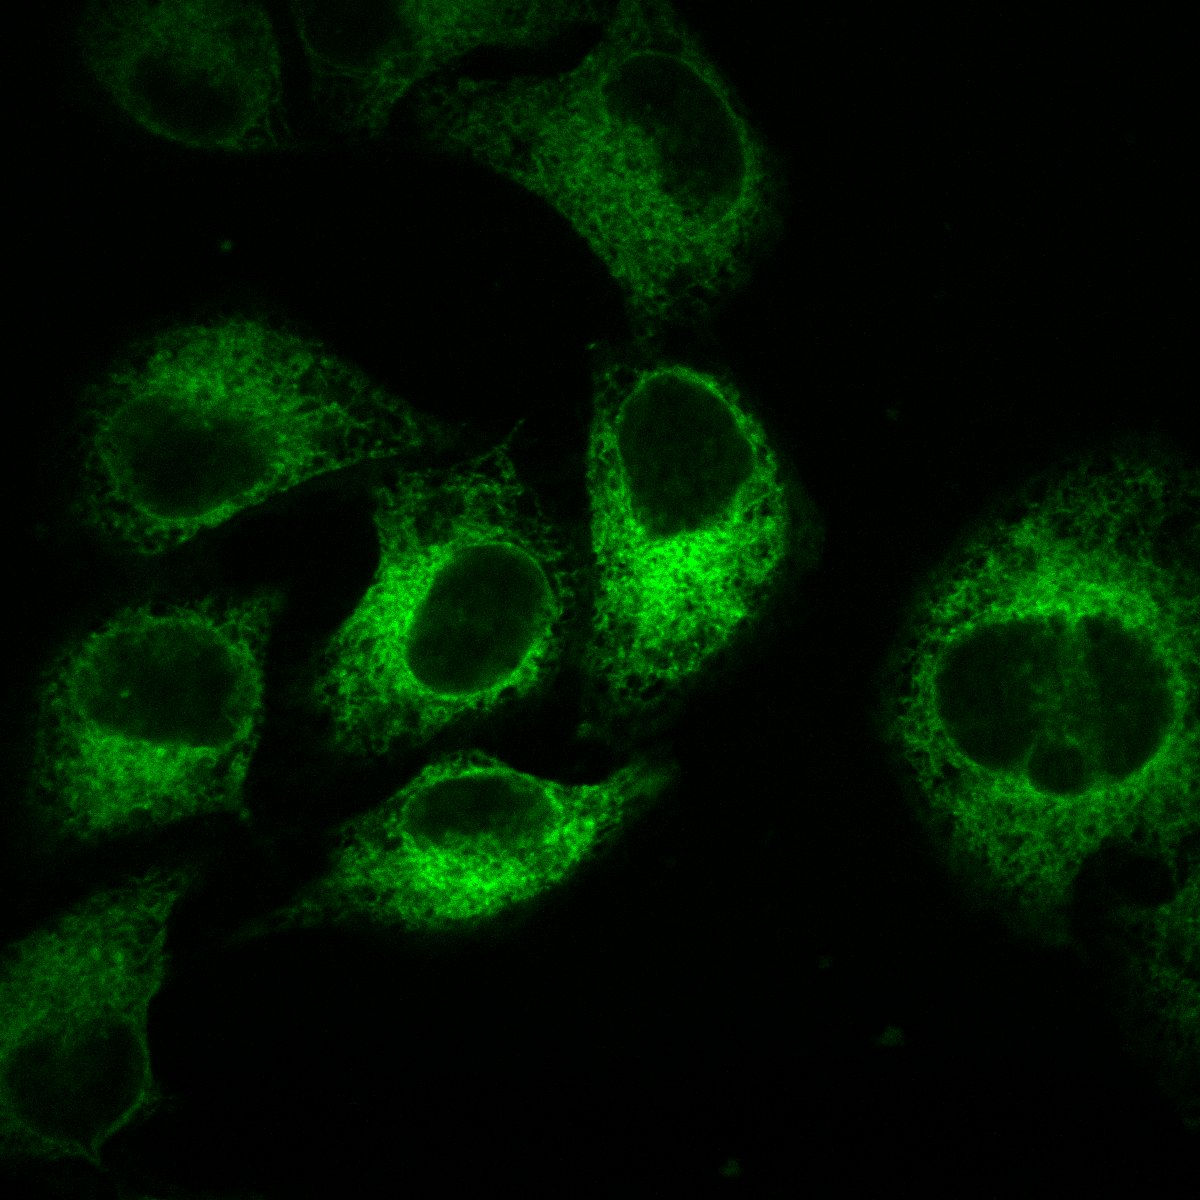
\includegraphics[width=0.3\linewidth]{../Figures/observations/G2 HeLa STING-GFP CON3.jpg}}
    \caption{Controlled Group}  
    \label{controlled group}
 \end{figure}

In controlled group, the fluorescence was equally and evenly distributed in cytosol except nucleus.
However, a few of unexpected cells (upper right corner of capture 2 in Figure \ref{controlled group}) appeared to be activated even without diABZI treatment.
Besides, we occasionally discovered several cells in division (may be telophase in mitotic phase).

\begin{figure}[h]
    \centering
    \subfigure[capture 1]{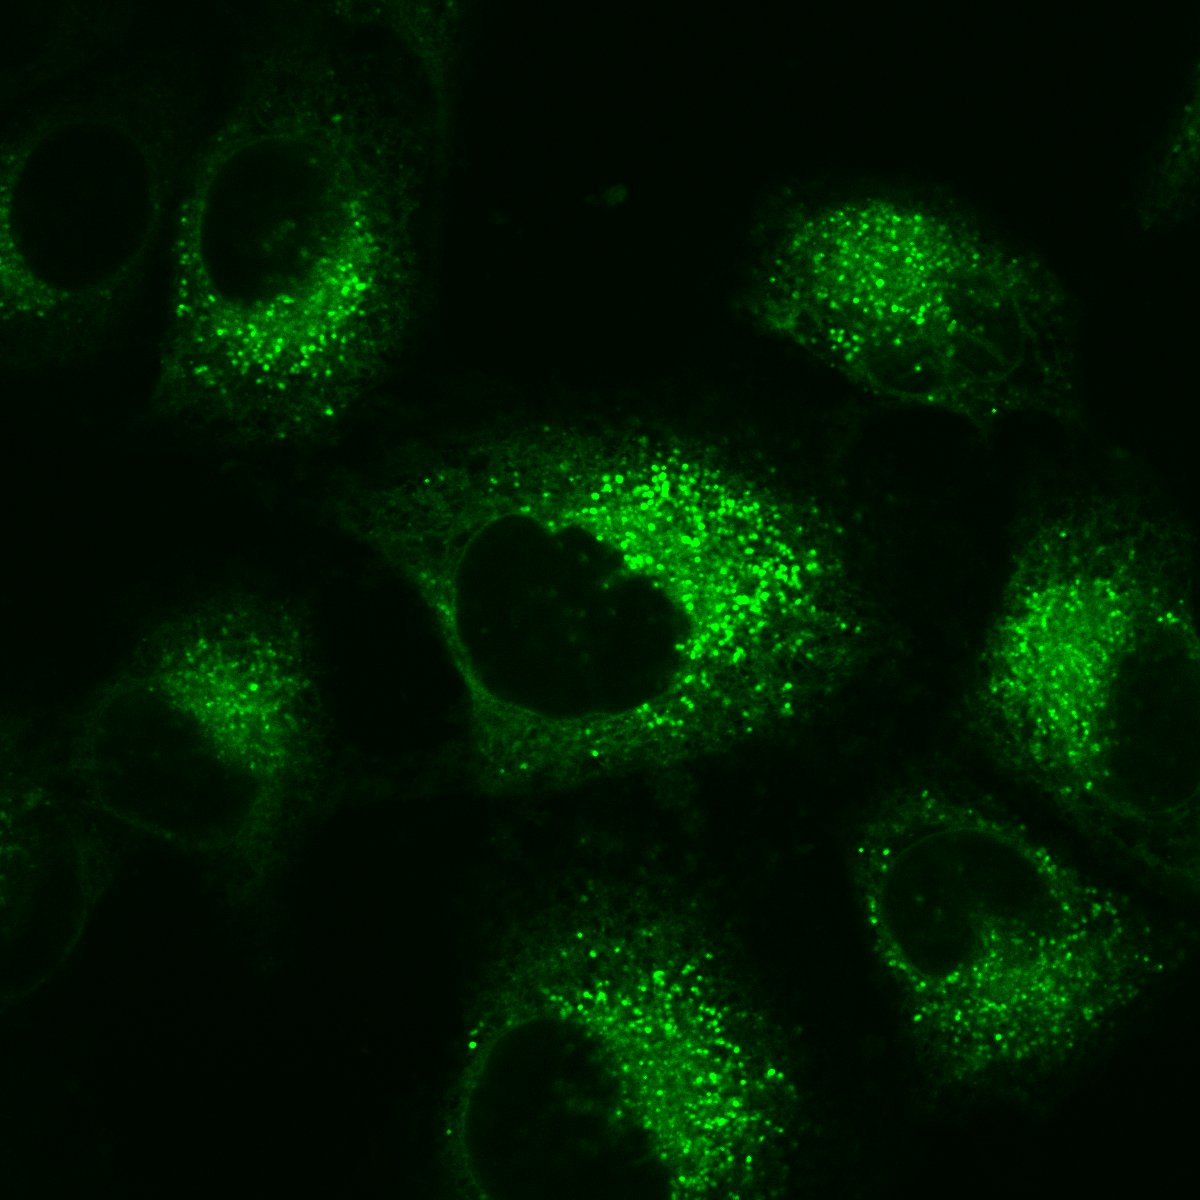
\includegraphics[width=0.3\linewidth]{../Figures/observations/G2 HeLa STING-GFP CON4.jpg}}
    \subfigure[capture 2]{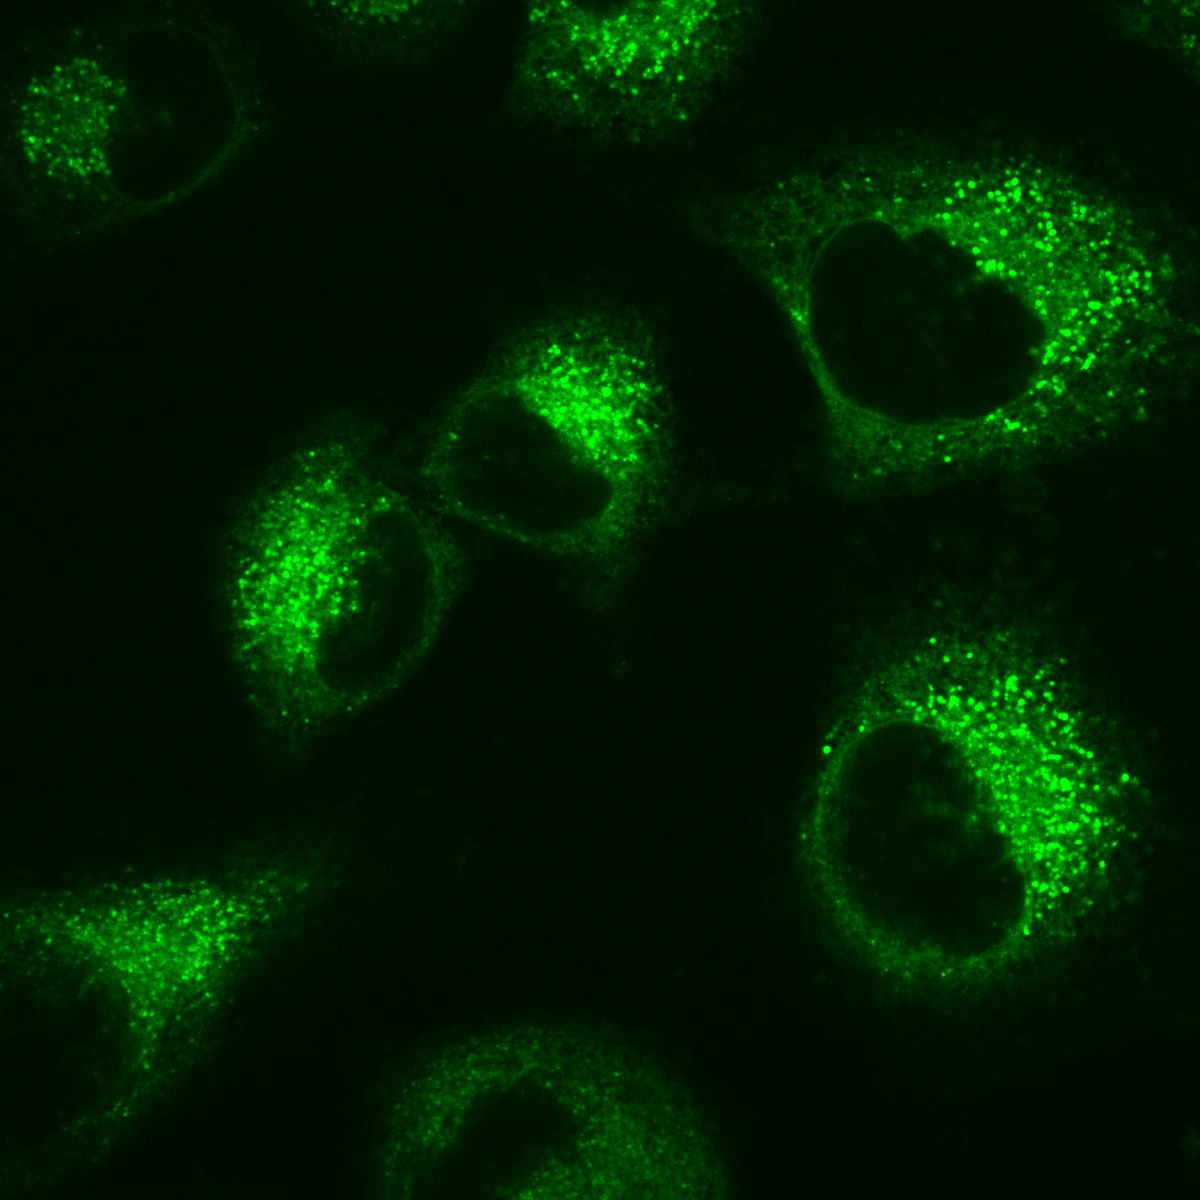
\includegraphics[width=0.3\linewidth]{../Figures/observations/G2 HeLa STING-GFP CON5.jpg}}
    \subfigure[capture 3]{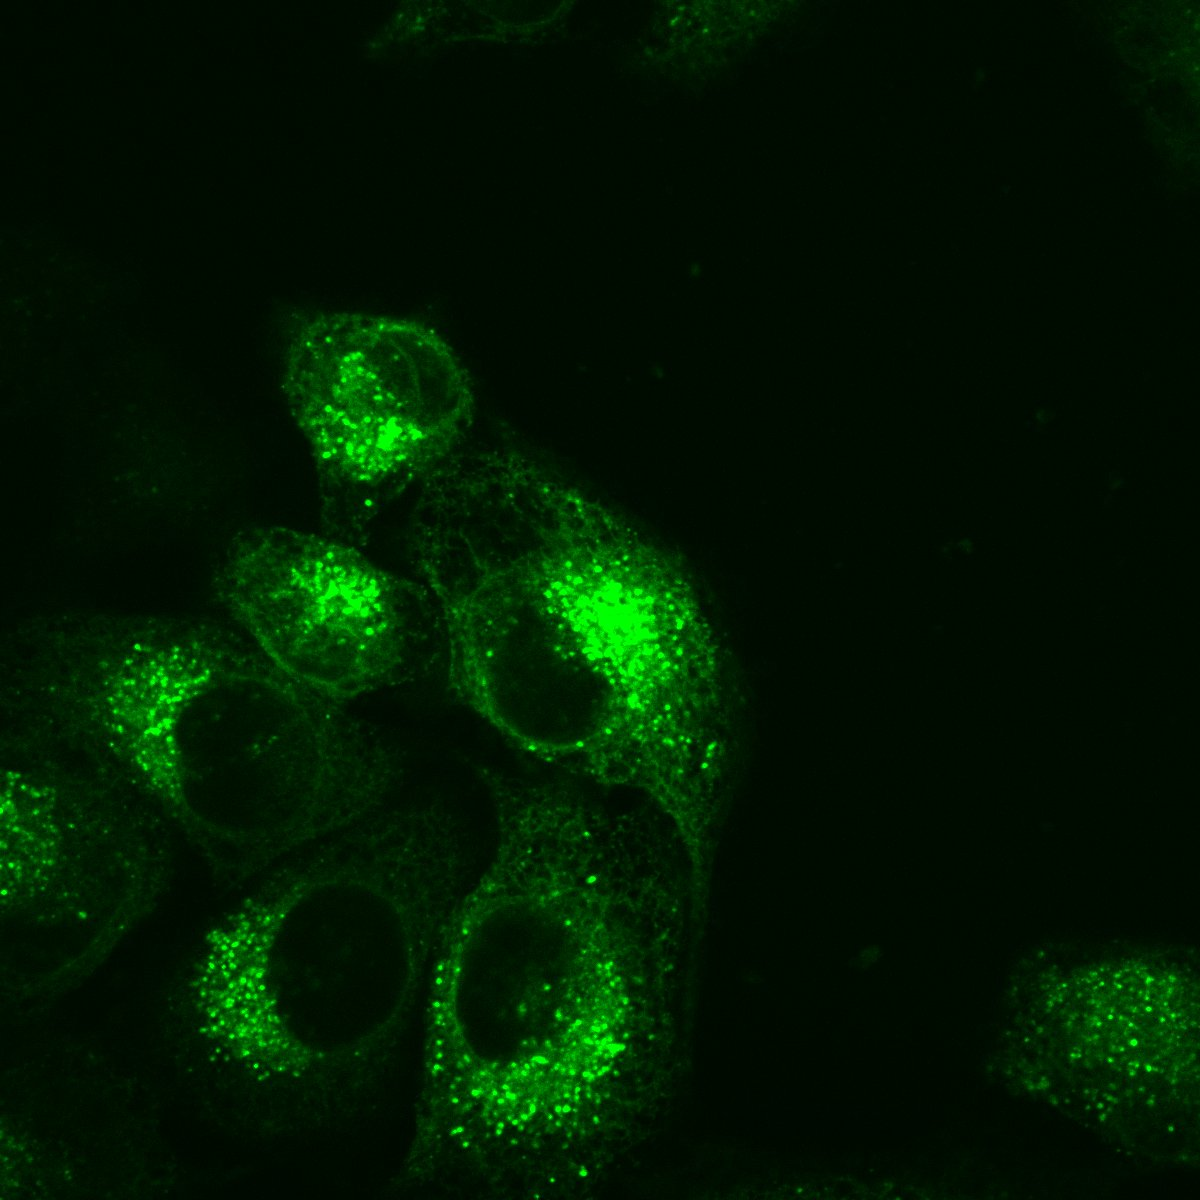
\includegraphics[width=0.3\linewidth]{../Figures/observations/G2 HeLa STING-GFP CON7.jpg}}
    \caption{Experimental Group (Treated by diABZI)}  
    \label{Experimental group}
 \end{figure}

 Compared with controlled group, the fluorescence distribution in each cell seemed to be more centered and much more bright forming a series of scatters.
 This phenomenon was consist with the theory of transportation of STING from ER to Golgi Apparatus or vesicular forming a concentrated separated phase here.

\section{Conclusion}
In this experiment we verified the transportation of STING protein from ER to Golgi Apparatus or vesicular, which is a critical step in cGAS-STING pathway of innate immune system.

The experiment acquainted us with fluorescence microscope and helped me to understand the importance as well as the mechanisms of innate immune system.
Thanks for the instructions from my teacher and teaching assistant.

\bibliographystyle{plain}
\bibliography{references}




\end{document}